\section{Appendix: Protocols of the Token Transaction Framework}

This appendix provides a high level description of the token transaction framework, including the data model, transaction flow, and cryptographic components. The protocol ensures privacy, security, and scalability by managing tokens off-chain while relying on coordination (Unicity) for single-spend proofs.


\subsection{Data Model}

\subsubsection{Token Structure}

A token \( T \) is a tuple defined as:
\[
T = (tokenId, tokenClass, tokenValue, \Gamma, \tau, S)
\]
where:
\begin{itemize}
	\item \( tokenId \): A unique 256-bit identifier for the token.
	\item \( tokenClass \): A unique 256-bit identifier for the token class (e.g., utility token, NFT).
	\item \( tokenValue \): A numeric value represented as a big integer.
	\item \( \Gamma \): The genesis state, containing minting proofs and data.
	\item \( \tau \): A sequence of transitions \( \tau = [t_1, t_2, \dots, t_n] \), where each \( t_i \) represents a state transition.
	\item \( S \): The current state of the token.
\end{itemize}


\subsubsection{Token State}

The state \( S \) of a token is defined as:
\[
S = (tokenId, tokenClass, pubkey, nonce)
\]
where:
\begin{itemize}
	\item \( pubkey \): The public key of the current owner.
	\item \( nonce \): A one-time random value used to ensure state uniqueness.
\end{itemize}


\subsubsection{Transition Structure}

A transition \( t \) is defined as:
\[
t = (sourceState, input, destinationState, salt)
\]
where:
\begin{itemize}
	\item\( sourceState \): The state before the transition.
	\item\( input \): The proof of ownership and Unicity proof.
	\item\( destinationState \): The state after the transition.
	\item\( salt \): A random value used to obfuscate the transaction digest.
\end{itemize}


\subsubsection{Transaction Structure}

A transaction \( tx \) is defined as:
\[
tx = (sourceState, input, destPointer, salt)
\]
where:
\begin{itemize}
	\item \( destPointer \): A pointer to the hidden destination state, shared by the recipient.
\end{itemize}


\subsection{Transaction Flow}

\subsubsection{Minting a Token}

\noindent\textbf{Inputs}:
\begin{itemize}
  \item \( secret \): A password to lock the token.
  \item \( tokenClass \): The token class (text string).
  \item \( tokenValue \): The token value (numeric).
\end{itemize}

\textbf{Process}:
\begin{itemize}
  \item Generate a unique \( tokenId \).
  \item Create the genesis state \( \Gamma \) with minting proofs.
  \item Lock the token to \( secret \).
  \item Submit a commit to the Unicity service to obtain a single-spend proof.
\end{itemize}

\noindent\textbf{Output}:
\begin{itemize}
  \item A token \( T \) with an initial state \( S \).
\end{itemize}


\subsubsection{Generating a Recipient Pointer}

\noindent\textbf{Inputs}:
  \begin{itemize}
    \item \( secret \): A password to lock the received token.
    \item \( nonce \): A one-time random value.
  \end{itemize}

\noindent\textbf{Process}:
  \begin{itemize}
    \item Compute the recipient's public key \( pubkey \) using \( secret \) and \( nonce \).
    \item Generate a pointer \( destPointer \) to the hidden destination state.
  \end{itemize}

\noindent\textbf{Output}:
  \begin{itemize}
    \item \( destPointer \): A pointer to the recipient's state.
  \end{itemize}


\subsubsection{Sending a Token}

\noindent\textbf{Inputs}:
  \begin{itemize}
    \item \( secret \): The password to unlock the token.
    \item \( destPointer \): The recipient's pointer.
  \end{itemize}

\noindent\textbf{Process}:
  \begin{itemize}
    \item Unlock the token using \( secret \).
    \item Create a transaction \( tx \) with the current state, \( destPointer \), and a random \( salt \).
    \item Submit the transaction commit to the Unicity gateway to obtain a single-spend proof.
    \item Update the token's state to reflect the pending transition.
  \end{itemize}

\noindent\textbf{Output}:
  \begin{itemize}
    \item A transaction \( tx \) with a Unicity proof.
  \end{itemize}

\subsubsection{Receiving a Token}

\noindent\textbf{Inputs}:
  \begin{itemize}
    \item \( secret \): The password to lock the received token.
    \item \( nonce \): The nonce used to generate the recipient's pointer.
  \end{itemize}

\noindent\textbf{Process}:
  \begin{itemize}
    \item Resolve the transaction \( tx \) into a transition \( t \) using \( nonce \) and \( secret \).
    \item Update the token's state to reflect the new ownership.
    \item Lock the token to \( secret \).
  \end{itemize}

\noindent\textbf{Output}:
  \begin{itemize}
    \item A token \( T \) with an updated state \( S \).
  \end{itemize}


\begin{figure}[!htbp]
    \begin{center}
    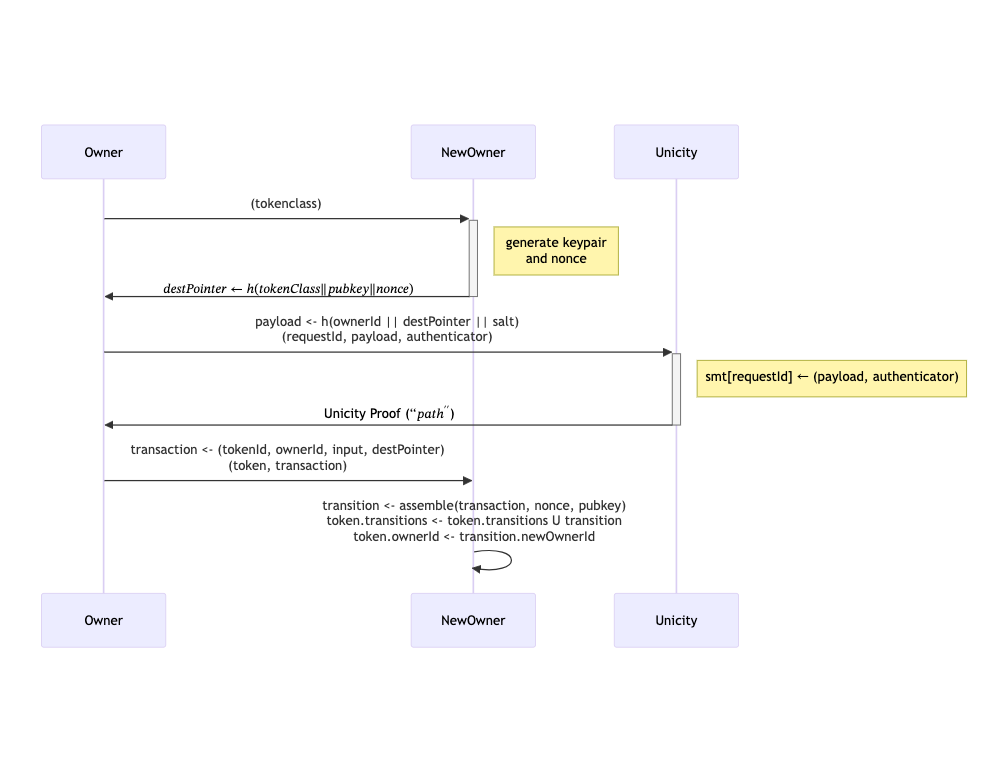
\includegraphics[width=\textwidth]{unicity-tx}
    \caption{Data flow of a Transaction}\label{fig:tx}
    \end{center}
\end{figure}
% https://mermaid.live/edit#pako:eNp9U8Fu2zAM_RVBMFAbc7q7UeSyXXJYW2DoZdOAKhZjC7UlV6JRBIn_fZSsOG47zBdLJB8f-SieeG0V8Ip7eB3B1PBdy8bJXhhG38ObAbfZbr_cw1s8VyxH-0JxnfS-mIPuLQJzummR2QO7RjZAP0m-FzgOUru7vfu6lUYxY4knYVM0cWwSLMuE6CW2_nBS4PHRaoPgJiZEA-hZmy_uWMm3UEnwntniGMY9cX4wRtapoPTvW3syutZ4rNggj52Vit1tiMQG906x85mtqghXLzssYi-5C5p53KnyAi6ZHLEFg7qWaN0_FVoIfY-_lxR_YuOhxSxj-X_TpQQrzZKFPTpLBPlKwufngQ43N1OWFe8bvw4KnTRe1qitCc3PEw5NJRFKps0wYrlWIikQQ8t1huLTYD8Q6QsPzQ36fQf5Cl3Oj4P0jCOcWSLJ7RXsA_qz8WmVf4W7TDJgFv-tSUXtlDC85D24XmpFe3AK9QtOqvcgeEVHBQc5dii4MBOF0kTsz6OpeYVuhJI7OzYtrw6y83QbB0VPPi3RYh2k-WXt9Q5K0zh_zJsXF3D6C_AtPcg


\subsection{Cryptographic Components}

\subsubsection{Unicity Proof}

The Unicity proof ensures that a token state is spent only once. It is represented as:
\[
\Pi = (requestId, payload, authenticator)
\]
where:
\begin{itemize}
  \item\( requestId \): A unique identifier derived from the token state.
  \item\( payload \): The digest of the transaction.
  \item\( authenticator \): A signature proving the commit's authenticity.
\end{itemize}

\subsubsection{Ownership Proof}

The ownership proof is a digital signature demonstrating knowledge of the private key corresponding to the public key in the token state:
\[
\sigma = Sign(sk, H(tokenId || tokenClass || pubkey || nonce))
\]
where \( sk \) is the private key of the owner.


\subsubsection{Commitment Scheme}

The commitment \( C \) for a transaction is computed as:
\[
C = H(requestId || payload || authenticator)
\]
where \( H \) is a cryptographic hash function.

\subsubsection{Pointer Obfuscation}

The recipient's pointer \( destPointer \) is computed as:
\[
destPointer = H(pubkey || nonce || salt)
\]
This ensures that the pointer reveals no information about the recipient's state.


\subsection{Security Properties}

\begin{description}
  \item[Single-Spend Guarantee:] The Unicity proof ensures that no two transitions can be created from the same state.
  \item[Privacy:] Token states, transactions, and commitments are obfuscated to prevent linkage to specific tokens or owners.
  \item[Ownership:] Only the owner with the correct private key can create valid transitions.
  \item[Scalability:] Commitments are aggregated into a distributed hash tree, enabling high throughput.
\end{description}

% \subsection{Example Workflow}

% \noindent\textbf{Minting}:
%   \begin{itemize}
%     \item User1 mints a token \( T \) with \( tokenId = id_1 \), \( tokenClass = C \), and \( tokenValue = V \).
%   \end{itemize}

% \noindent\textbf{Generating Pointer}:
%   \begin{itemize}
%     \item User2 generates a pointer \( destPointer = ptr_2 \) using \( nonce = n_2 \) and \( secret = s_2 \).
%   \end{itemize}

% \noindent\textbf{Sending}:
%   \begin{itemize}
%     \item User1 sends \( T \) to \( ptr_2 \) by creating a transaction \( tx \).
%   \end{itemize}

% \noindent\textbf{Receiving}:
%   \begin{itemize}
%      \item User2 resolves \( tx \) into a transition \( t \) and updates \( T \) to reflect the new ownership.
%   \end{itemize}

